\newcommand{\sigmatwo}{\overline{\sigma}}
The current query evaluation mechanism for \datalogM is a bottom-up naive\cite{Green:2013:DRQ:2688167.2688168} evaluation. It is based on the fixpoint-theoretic semantics that derives tuples from rules until no new tuples can be derived. The rule evaluation is performed using relational algebra (see e.g. \cite{Abiteboul:1995:FDL:551350}) and a thorough description is given in Appendix A.

\subsection{Mutual Dependencies and Predicate Ordering}
With multiple rules and potentially many mutual dependencies between the predicates, there is a need to find an order in which to apply the rules. Indeed, for mutually dependent predicates, all rules that may derive new facts for those predicates need to be iterated together. \textit{Stratification}\cite{Green:2013:DRQ:2688167.2688168} is the process of clustering the predicates that need to be computed together into so called \textit{strata} as well as to find an optimal order between the strata. The iterative fix-point algorithm is then run over each \textit{stratum} following the computed order. The process is formalized below.

A predicate $P_i$ \textit{directly depends} on predicate $P_j$ iff there exists a rule for which $P_i$ is in the head and $P_j$ is in the body. Let $Dep(P_i)$ be the set of predicates which $P_i$ directly depends on. The dependency graph $G_{DEP}$ has the set of predicate symbols as vertices and there is an edge from $P_i$ to $P_j$ iff $P_j \in DEP(P_i)$. A strongly connected component in $G_{DEP}$ then contains the predicates which are mutually recursive. Such a connected component can be found e.g. using Tarjan's algorithm \cite{Tarjan72depthfirst} and is called a stratum. By merging the vertices of $G_{DEP}$ into such strata we get a graph $G_{STRAT}$ with vertices being the strata of $G_{DEP}$ and edges the collapsed multi-edges from $G_{DEP}$. By construction there exists a total order on $G_{STRAT}$ with $S_1 < S_2$ iff $(S_1, S_2) \in Edge(G_{STRAT})$. The desired order is found by a reverse post-order search of $G_{STRAT}$.
\begin{figure*}[!hbt]
	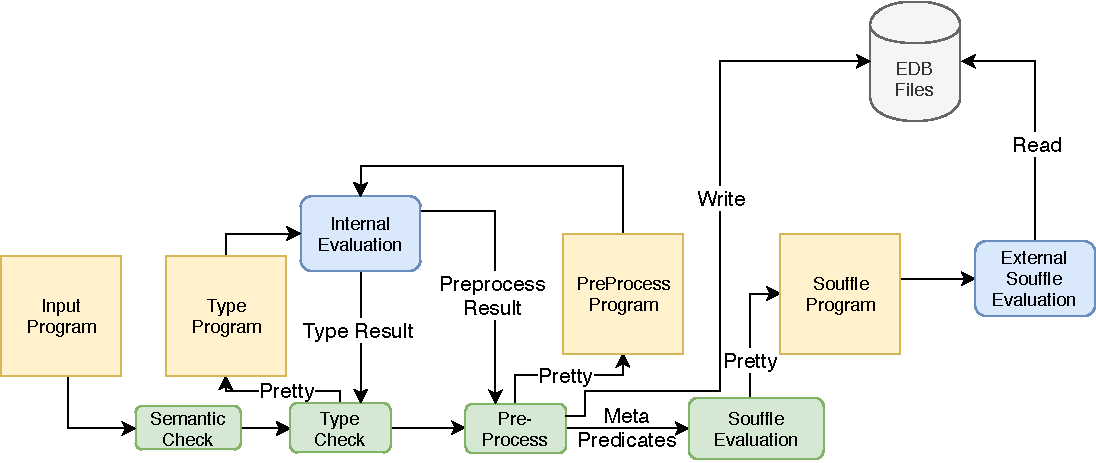
\includegraphics[scale=0.7]{img/souffleEval.pdf}
	\caption{Souffle Printing Pipeline. \textbf{Yellow}: A Datalog Program. \textbf{Blue}: An evaluation mechanism. \textbf{Green}: A compiler stage. }
	\label{figure:soufflePipeline}
\end{figure*}
\subsection{Cross Compilation}
In addition to internal evaluation, $Datalog^M$ supports cross-compilation, or pretty-printing, to Souffle\cite{SouffleHome}. The compilation pipeline is shown in figure \ref{figure:soufflePipeline}. First, a number of semantic checks are performed. For example, the semantic check ensures that all variables used in the head of a rule also occures in the body of the rule (the range restriction property\cite{Ceri:1989:YAW:627272.627357}). In the next stage, the program is type checked (type-checking is described in more detail in the following section). As was mentioned in the introduction (and will be explained in the next section), \datalogM supports meta-predicates. Souffle however has no such support so naturally it does not recognize the meta-semantics. To this end, a separate pre-process Datalog program is generated to evaluate all meta-predicates and subsequently output them as EDB files. Finally, the program is pretty-printed to a Souffle program $P_{Souffle}$. $P_{Souffle}$ declares the meta-predicates and loads them from the EDB files; the meta-predicates can then be used as ordinary predicates within the Souffle environment.